%From https://egu2018.eu/PICO_how-to_guide_to_PICO.pdf
%Abstracted and templated by Brian Ballsun-Stanton, Macquarie University.
%original template by https://github.com/snowtechblog/pico-latex-presentation by Anselm Köhler

\documentclass[unknownkeysallowed,usepdftitle=false, parskip=full, aspectratio=169]{beamer}
% unknownkeysallowed is needed for mac and the newer latex version -> is more picky than before...
\usetheme[headheight=1cm,footheight=2cm]{boxes}
%\usetheme{default}


\usepackage{default}
\usepackage{graphicx}
%example pictures created via: http://lorempixel.com/1200/800/cats/Figure2/. Credit to http://lorempixel.com/images.php

\usepackage{epsfig}
\usepackage{siunitx}
\usepackage{color}
\usepackage{ifthen}
%usepackage{ragged2e}

\usepackage[T1]{fontenc}
\usepackage[utf8]{inputenc}
%https://tex.stackexchange.com/a/203804/5483

\usepackage[activate={true,nocompatibility},final,tracking=true,kerning=true,spacing=true,factor=1100,stretch=10,shrink=10]{microtype} % http://www.khirevich.com/latex/microtype/
\microtypecontext{spacing=nonfrench}

\usepackage{lipsum} % for dummy text only
\usepackage[UKenglish]{babel} %https://tex.stackexchange.com/a/27743 
\usepackage[pangram]{blindtext} % https://tex.stackexchange.com/a/48411

%\usepackage{parskip} % from https://tex.stackexchange.com/q/11622
%\setlength{\parskip}{12pt} 

%\setparsizes{\parindent}{12pt}{\parfillskip}

%\usepackage{etoolbox} % as per https://tex.stackexchange.com/a/24331
%\appto\chapterheadendvskip{\vspace{-1\parskip}}
%\setparsizes{\parindent}{50pt plus 20pt minus 30pt}{\parfillskip}

\setbeamertemplate{navigation symbols}{}%remove navigation symbols
\setbeamersize{text margin left=1cm,text margin right=1cm}

% some colors
\definecolor{grau}{gray}{.5}
\definecolor{slfcolor}{rgb}{0,0.6274,0.8353}
\definecolor{wslcolor}{rgb}{0,0.4,0.4}

% setup links
\hypersetup{%
	%linkbordercolor=green,%
	colorlinks=false,%
	pdfborderstyle={/S/U/W 0},%
	%pdfpagemode=FullScreen,%
	pdfstartpage=4%
	}

% setup some fonts
\setbeamerfont{title}{series=\bfseries, size=\small}
\setbeamerfont{author}{size*={5pt}{0pt}}
\setbeamerfont{institute}{size*={3pt}{0pt}}
\setbeamerfont{bodytext}{size=\scriptsize}
\setbeamerfont{caption}{size*={0.1pt}{0.0pt}}
	
% Title setup	
\title{Improving the Organisation of Sources and References}
\author{Osmond Chiu\inst (\texttt{osmond.chiu@student.mq.edu.au})}
\institute{Macquarie University}
% add title in headbox
\setbeamertemplate{headline}
{\leavevmode
\begin{beamercolorbox}[width=1\paperwidth]{head title}
  % LOGO
  \vspace{0.1cm}
  \begin{columns}[t, totalwidth=\textwidth]
  \begin{column}[c]{1.05cm}
  \end{column}
  % TITLE
   \begin{column}[c]{10.6cm}
   \centering \usebeamerfont{title} \textcolor{red}{\inserttitle} \\
   \centering \usebeamerfont{author} \color[rgb]{0,0,0} \insertauthor \\
   \vspace{-0.05cm}
   \centering \usebeamerfont{institute} \insertinstitute
  \end{column}
  % PICTURE
  \begin{column}[c]{1.15cm}
    \hspace{0.005cm}
  \end{column}
  \end{columns}
  {\color{red}\hrule height 1pt\vspace{0.1cm}}
\end{beamercolorbox}%
}

% setup the navigation in footbox
% first set some button colors
\newcommand{\buttonactive}{\setbeamercolor{button}{bg=red,fg=white}}
\newcommand{\buttonpassive}{\setbeamercolor{button}{bg=red,fg=black}}
% now set up that the one active one gets the new color.
\newcommand{\secvariable}{nothing}
% therefore we write before each section (well, everything which should be part of the navi bar)
% the variable \secvariable to any name which is in the next function ...
\newcommand{\mysection}[1]{\renewcommand{\secvariable}{#1}
}
% ... compaired to strings in the following navibar definition ...
\newcommand{\tocbuttoncolor}[1]{%
 \ifthenelse{\equal{\secvariable}{#1}}{%
    \buttonactive}{%
    \buttonpassive}
 }
% ... here we start to set up the navibar. each entry is calling first the function \tocbuttoncolor with the argument which should be tested for beeing active. if active, then change color. afterwards the button is draw. so to change that, you need to change the argument in \toc..color, the first in \hyperlink and before each frames definition... A bit messed up, but works...
\newlength{\buttonspacingfootline}
\setlength{\buttonspacingfootline}{-0.2cm}
\setbeamertemplate{footline}
{\leavevmode
\begin{beamercolorbox}[width=1\paperwidth]{head title}
  {\color{red}\hrule height 1pt}
  \vspace{0.05cm}
  % set up the buttons in an mbox
  \centering \mbox{
    \tocbuttoncolor{abstract}
    \hyperlink{abstract}{\beamerbutton{2 Min Madness}}
    \tocbuttoncolor{radar}
    \hspace{\buttonspacingfootline}
      \hyperlink{radar}{\beamerbutton{Functions}}

    \tocbuttoncolor{line}
    \hspace{\buttonspacingfootline}
      \hyperlink{line}{\beamerbutton{VirtualBox}}
    \tocbuttoncolor{major}
    \hspace{\buttonspacingfootline}
      \hyperlink{major}{\beamerbutton{Open Semantic}}
    \tocbuttoncolor{slab}
    \hspace{\buttonspacingfootline}
      \hyperlink{slab}{\beamerbutton{Zotero}}
    \tocbuttoncolor{minor}
    \hspace{\buttonspacingfootline}
      \hyperlink{minor}{\beamerbutton{Hypothes.is}}
    \tocbuttoncolor{conclusion}
    \hspace{\buttonspacingfootline}
      \hyperlink{conclusion}{\beamerbutton{Conclusion}}
    % this last one should normaly not be used... it will open the preferences to change the 
    % behaviour of the acrobat reader in fullscreen -> usefull in pico...
    \setbeamercolor{button}{bg=white,fg=black}
    % for presentation
    %\hspace{-0.1cm}\Acrobatmenu{FullScreenPrefs}{\beamerbutton{\#}}
    % for upload
    
     
\Acrobatmenu{FullScreenPrefs}{\vspace{0.3cm}\hspace{0.24cm}\mbox{%
      
\includegraphics[height=0.04\textheight,keepaspectratio]{%
	  figure/CreativeCommons_Attribution_License.eps}%
	  }}
   }
    \vspace{0.05cm}
\end{beamercolorbox}%
}


\begin{document}


%%%%%%%%%%%%%%%%%%%%%%%%%%%%%%%%%%%%%%%%%%%%%%%%%%%%%%%%%%%%%%%%%%%%%%%%%%
\mysection{abstract}
%%%%%%%%%%%%%%%%%%%%%%%%%%%%%%%%%%%%%%%%%%%%%%%%%%%%%%%%%%%%%%%%%%%%%%%%%%
\begin{frame}\label{\secvariable}

\parbox{\linewidth}{

\begin{columns}[t]
    \begin{column}[c]{0.5\textwidth}

Organising sources and managing references are two common and time consuming tasks when doing research.

 \vspace{12pt}

Common problems with these tasks:
\begin{itemize}
\item Cannot remember relevant source
\item Cannot remember key line in source
\item Cannot recall the topics covered in a source
\item Need to double check citations
\item Need to keep track of references for a bibliography
\end{itemize}

 \end{column}
    \begin{column}[c]{0.5\textwidth}
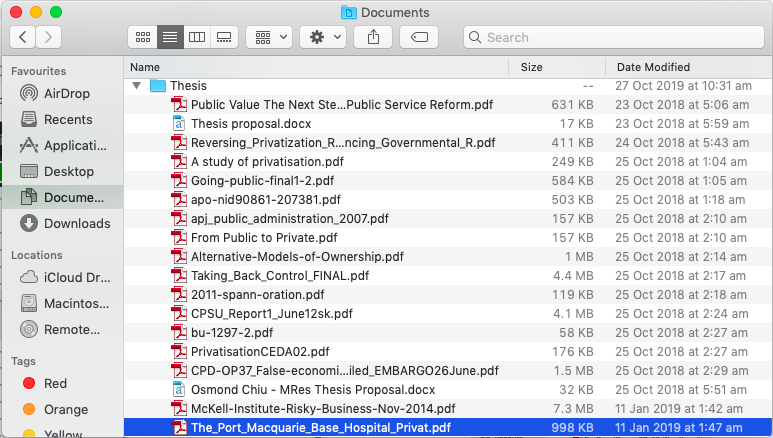
\includegraphics[width=1.5\textwidth,height=0.55\textheight,keepaspectratio]{figure/pdf.png}\\

\includegraphics[width=1.05\textwidth,height=0.5\textheight,keepaspectratio]{figure/bibliography.png}\\

 \vspace{12pt}


 
   \end{column}
  \end{columns}

}

   
\end{frame}

\begin{frame}\label{\secvariable}
  %https://tex.stackexchange.com/a/7452/5483
    \parbox{\linewidth}{

\begin{columns}[t]
\begin{column}[c]{0.5\textwidth}
      
      I have written an installer for MacOS so you can access three tools using \href{https://github.com/MQ-FOAR705/Osmond-Chiu---Proof-of-Concept---Implementation.git}{\textbf{one download}}.
 
      \vspace{12pt}
      
      Tool functions include annotation, tagging, a local search engine and reference management.
      
      \vspace{12pt}
 
      It will save you time on organising sources and managing references that could be better spent on improving your research!

 \end{column}
    \begin{column}[c]{0.5\textwidth}
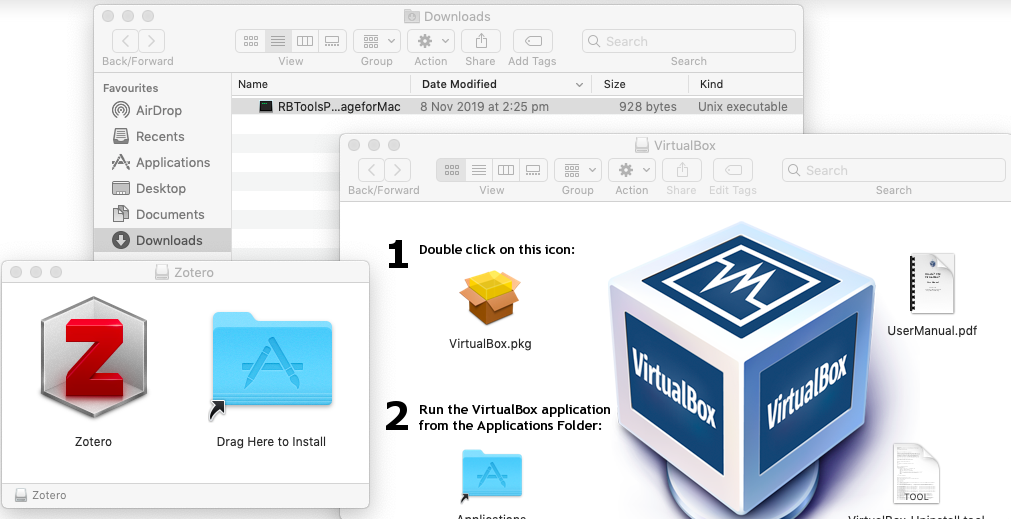
\includegraphics[width=1\textwidth,height=0.5\textheight,keepaspectratio]{figure/macos.png}\\
   \end{column}
  \end{columns}
}
 
\end{frame}

%%%%%%%%%%%%%%%%%%%%%%%%%%%%%%%%%%%%%%%%%%%%%%%%%%%%%%%%%%%%%%%%%%%%%%%%%%
\mysection{radar}
%%%%%%%%%%%%%%%%%%%%%%%%%%%%%%%%%%%%%%%%%%%%%%%%%%%%%%%%%%%%%%%%%%%%%%%%%%
\begin{frame}\label{\secvariable}

What tools comprises the software package?

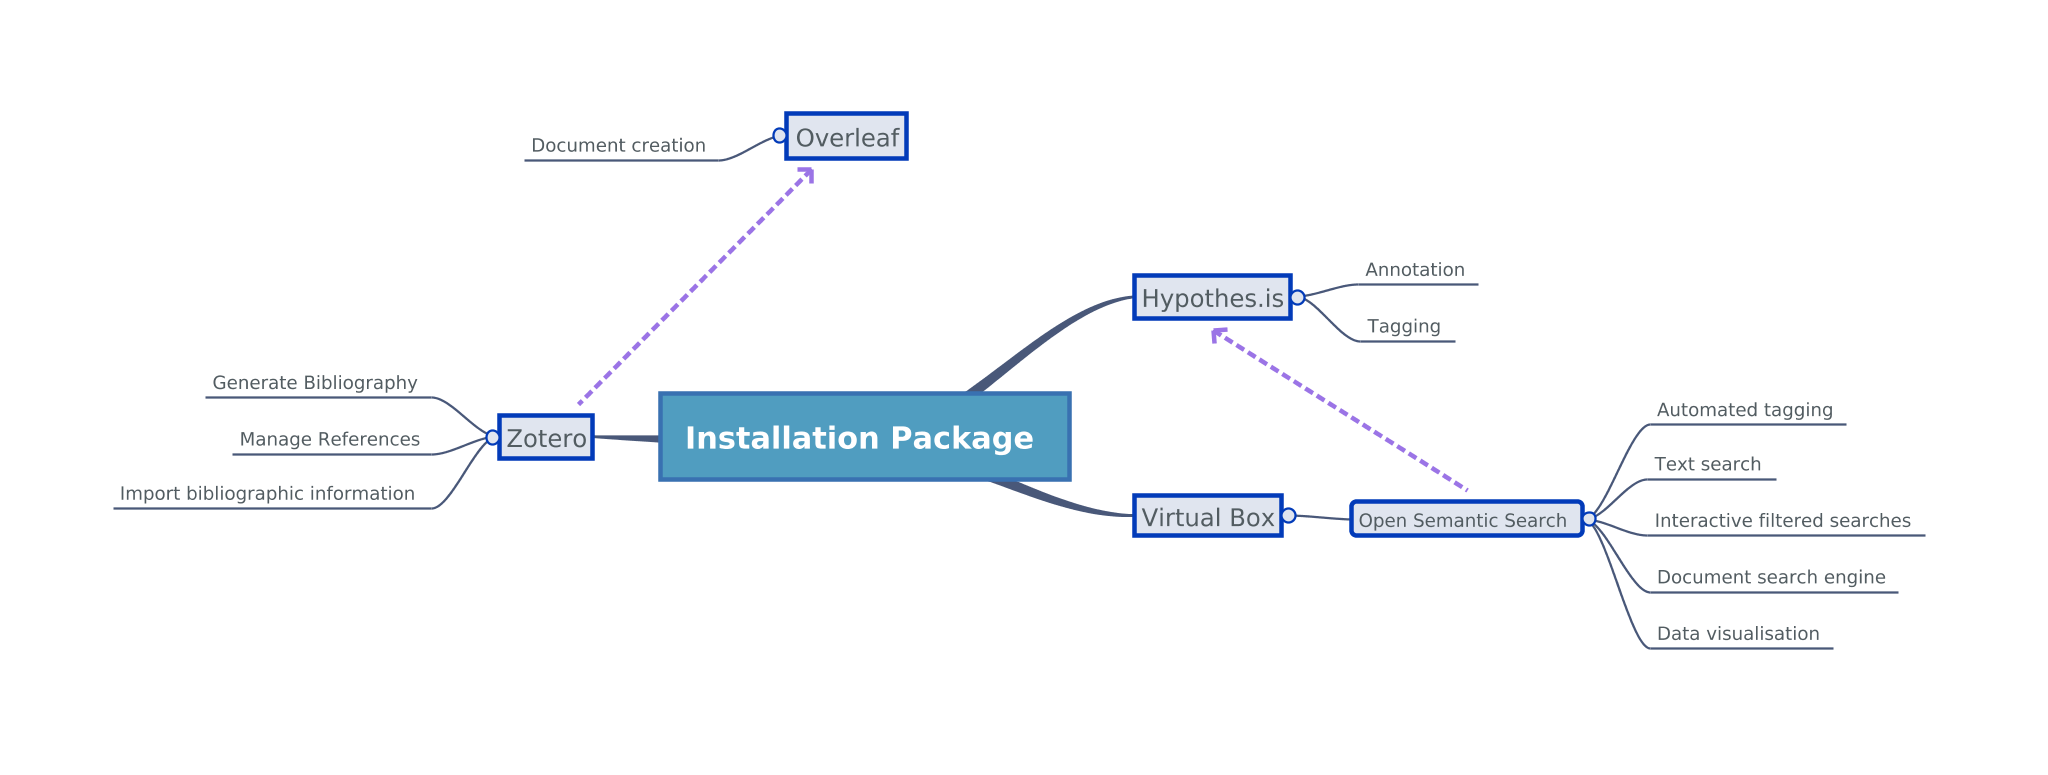
\includegraphics[width=2\textwidth,height=0.8\textheight,keepaspectratio]{%
figure/Pico.png}\\Three tools for any researcher: \textbf{Zotero}, \textbf{Hypothes.is} and \textbf{Open Semantic Search}.

\end{frame}

%%%%%%%%%%%%%%%%%%%%%%%%%%%%%%%%%%%%%%%%%%%%%%%%%%%%%%%%%%%%%%%%%%%%%%%%%%
\mysection{line}
%%%%%%%%%%%%%%%%%%%%%%%%%%%%%%%%%%%%%%%%%%%%%%%%%%%%%%%%%%%%%%%%%%%%%%%%%%
\begin{frame}\label{\secvariable}

  \begin{columns}[t]
  %https://tex.stackexchange.com/a/7452/5483
  \begin{column}[c]{0.3\textwidth}
\textbf{VirtualBox} enables you to create a Virtual Machine where you can run another Operating System.\par
\vspace{0.5cm}
VirtualBox is a requirement for Open Semantic Search.

    \end{column}
    \begin{column}[c]{0.7\textwidth}
    \parbox{\linewidth}{
  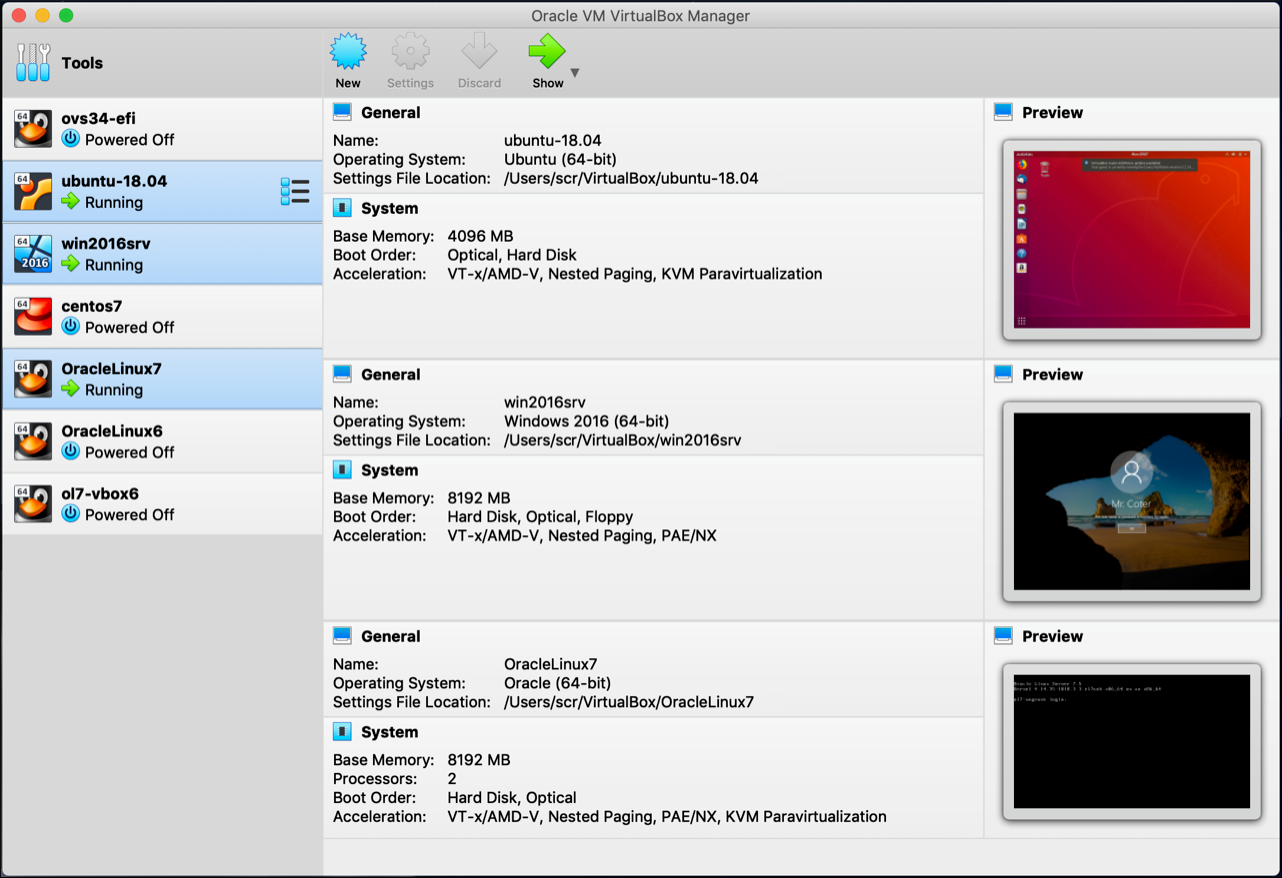
\includegraphics[width=1.7\textwidth,height=0.8\textheight,keepaspectratio]{%
figure/VirtualBox.png}\\  

}
    \end{column}
    
  \end{columns}


\end{frame}


%%%%%%%%%%%%%%%%%%%%%%%%%%%%%%%%%%%%%%%%%%%%%%%%%%%%%%%%%%%%%%%%%%%%%%%%%%
\mysection{major}
%%%%%%%%%%%%%%%%%%%%%%%%%%%%%%%%%%%%%%%%%%%%%%%%%%%%%%%%%%%%%%%%%%%%%%%%%%
\begin{frame}\label{\secvariable} %%Eine Folie
%http://lorempixel.com/1200/800/cats/Figure5/

\textbf{Open Semantic Search} is an integrated research tools for easier searching, monitoring, analytics, discovery and text mining of large document sets.
  \vspace{0.5cm}

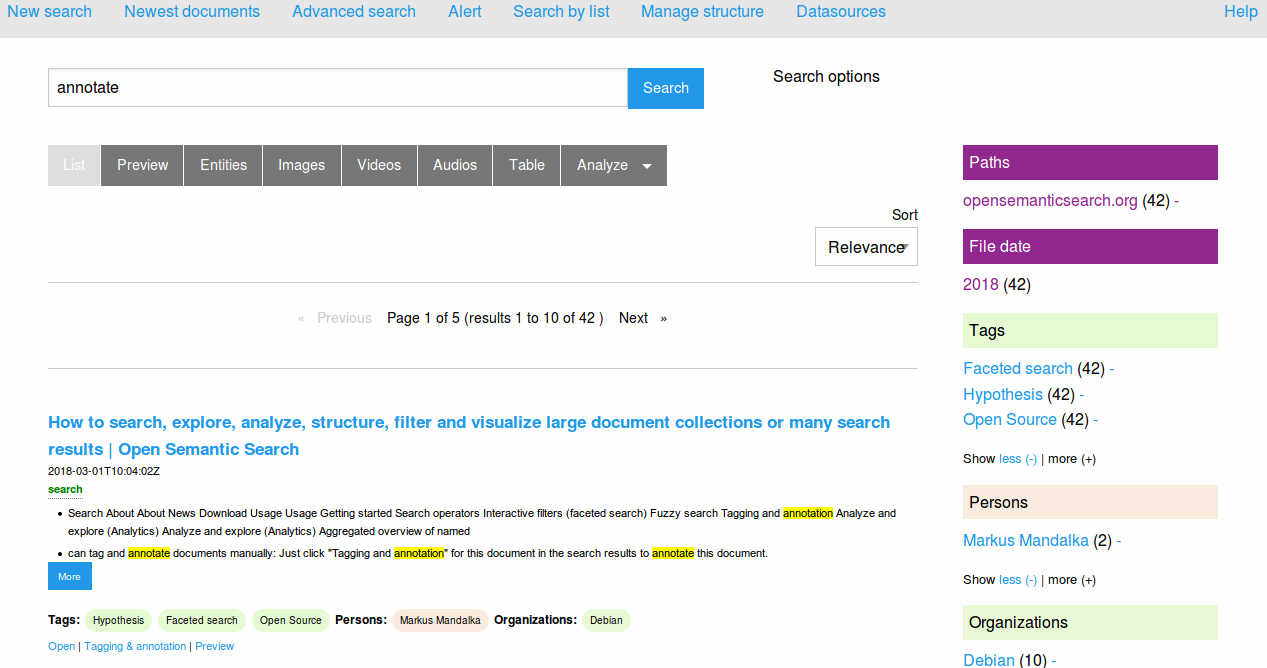
\includegraphics[width=1\textwidth,height=0.8\textheight,keepaspectratio]{%
figure/search.png} 


\end{frame}

\begin{frame}

Documents are indexed and can also be tagged and annotated to improve the organisation of data sources.
  \vspace{0.5cm}

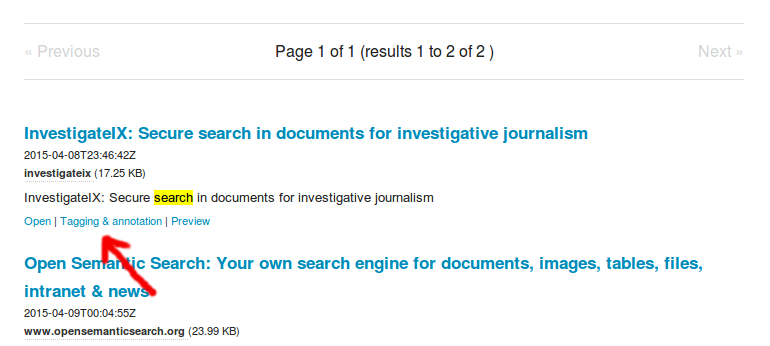
\includegraphics[width=1.1\textwidth,height=0.55\textheight,keepaspectratio]{%
figure/OpenSemantictagging.png} 
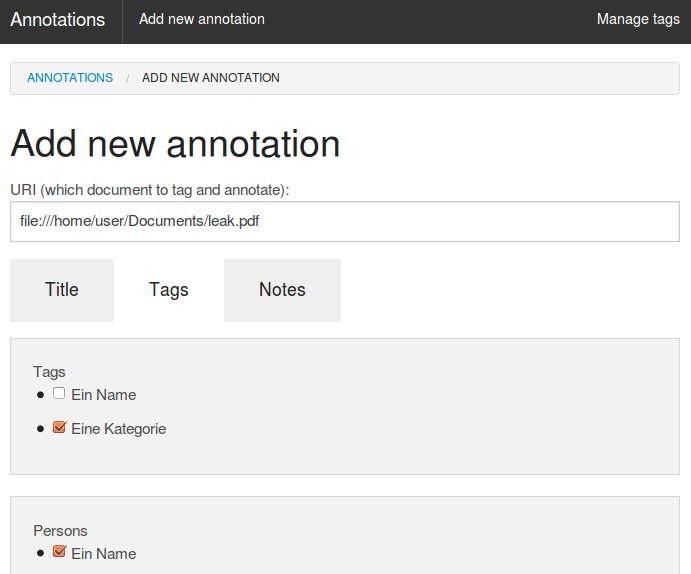
\includegraphics[width=1.1\textwidth,height=0.55\textheight,keepaspectratio]{%
figure/OpenSemanticannotation.png}  

\begin{columns}
\begin{column}[t]{1.1\textwidth}
\end{column}
\end{columns}


\end{frame}

%%%%%%%%%%%%%%%%%%%%%%%%%%%%%%%%%%%%%%%%%%%%%%%%%%%%%%%%%%%%%%%%%%%%%%%%%%
\mysection{slab}
%%%%%%%%%%%%%%%%%%%%%%%%%%%%%%%%%%%%%%%%%%%%%%%%%%%%%%%%%%%%%%%%%%%%%%%%%%

\begin{frame}\label{\secvariable}
  \begin{columns}[t]
  %https://tex.stackexchange.com/a/7452/5483
  \begin{column}[c]{0.3\textwidth}
\textbf{Zotero} can store, manage, and cite bibliographic references, such as books and articles.\par
  \vspace{6pt}
It syncs to an online account that can be used on different computers and links to Word and typesetting programs such as Overleaf.
    \end{column}
    \begin{column}[c]{0.7\textwidth}
    \parbox{\linewidth}{
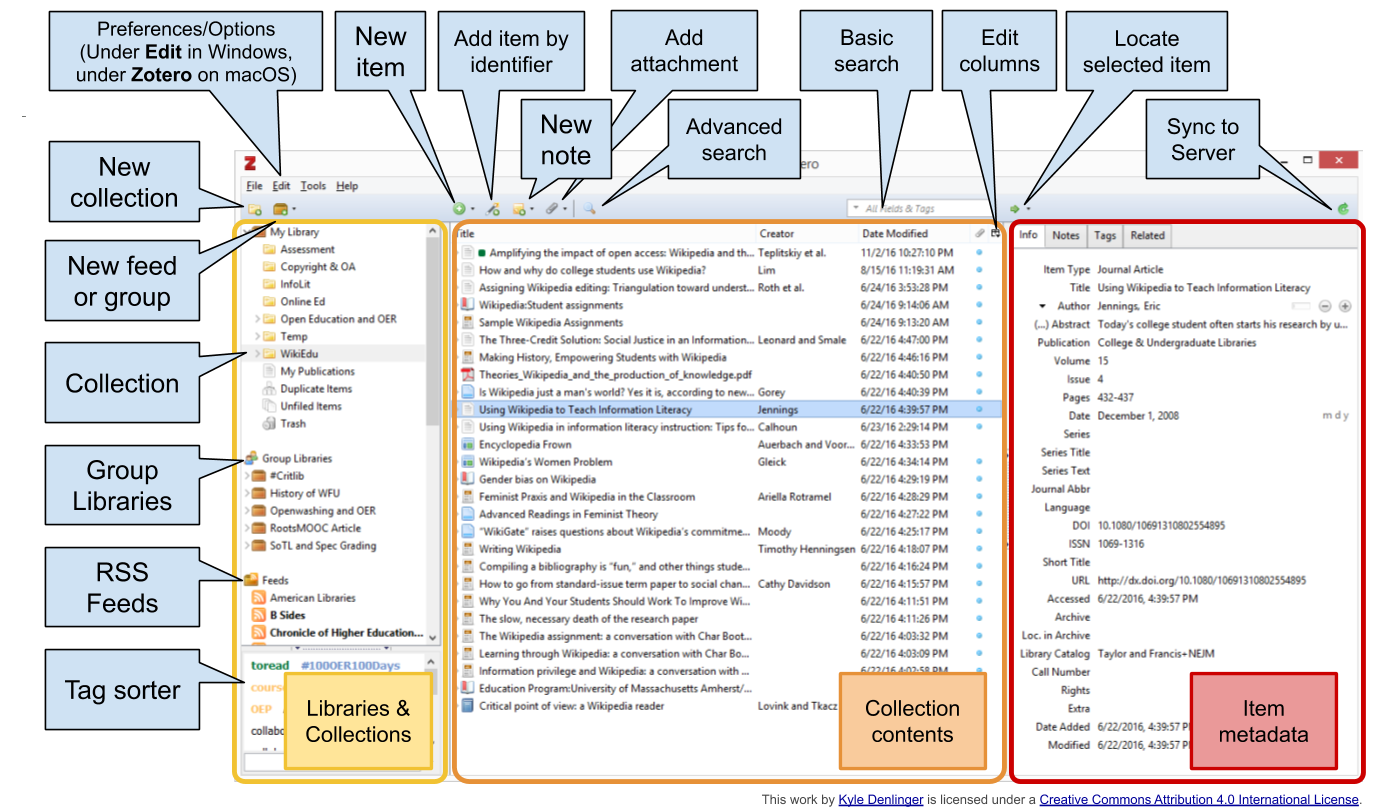
\includegraphics[width=1\textwidth,height=0.75\textheight,keepaspectratio]{%
figure/ZoteroFunctions.png}

}
    \end{column}
    
  \end{columns}


\end{frame}






%%%%%%%%%%%%%%%%%%%%%%%%%%%%%%%%%%%%%%%%%%%%%%%%%%%%%%%%%%%%%%%%%%%%%%%%%%
\mysection{minor}
%%%%%%%%%%%%%%%%%%%%%%%%%%%%%%%%%%%%%%%%%%%%%%%%%%%%%%%%%%%%%%%%%%%%%%%%%%

\begin{frame}\label{\secvariable}
  \begin{columns}[t]
  %https://tex.stackexchange.com/a/7452/5483
  \begin{column}[c]{0.45\textwidth}
%http://lorempixel.com/1200/800/cats/Figure2/     
%http://lorempixel.com/1200/800/cats/Figure3/
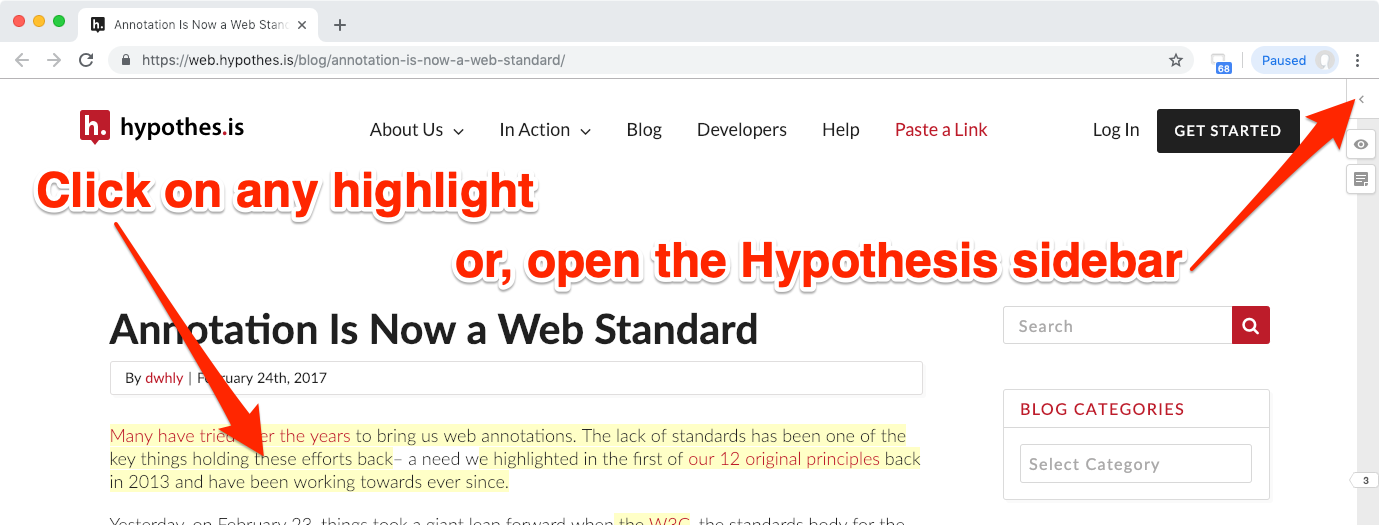
\includegraphics[width=0.8\textwidth,height=0.4\textheight,keepaspectratio]{%
figure/HypothesisHighlight.png}\\
\vspace{1pt}
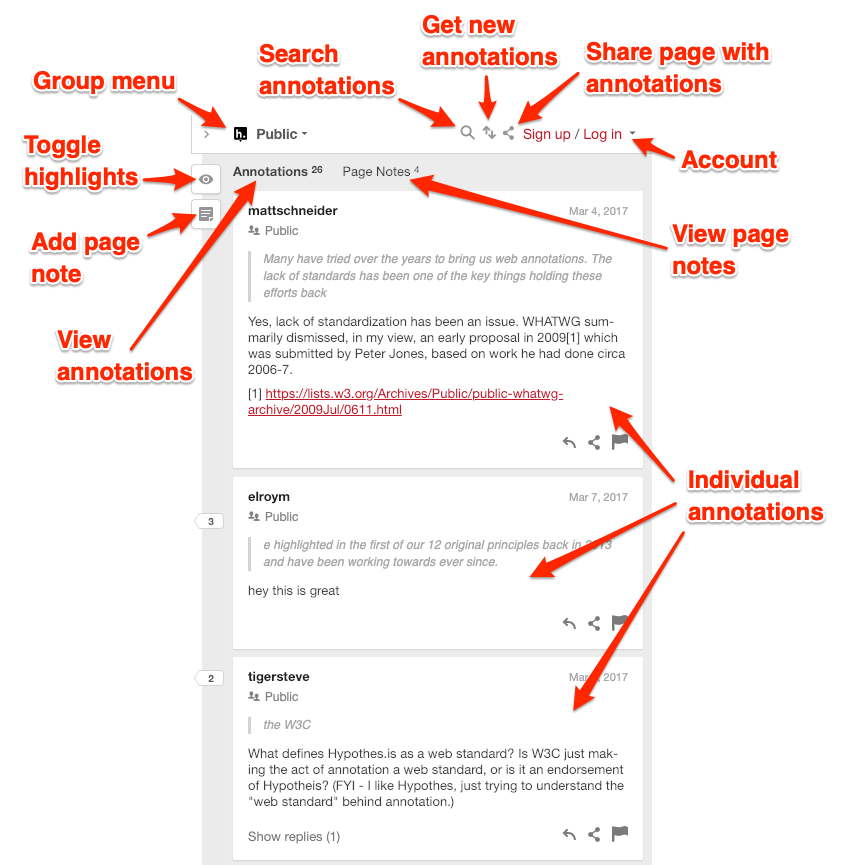
\includegraphics[width=1.5\textwidth,height=0.75\textheight,keepaspectratio]{%
figure/HypothesisAnnotate.png}
    \end{column}
    \begin{column}[c]{0.45\textwidth}
    \parbox{\linewidth}{

\textbf{Hypothes.is} is an annotation tool for digital documents.\par
\vspace{12pt}
Selected passages in documents viewed through an internet browser can be highlighted, notes can be added and tags generated.\par
\vspace{12pt}
Annotations can be grouped together, shared publicly or privately and searched through. 
}
    \end{column}
    
  \end{columns}


\end{frame}

%%%%%%%%%%%%%%%%%%%%%%%%%%%%%%%%%%%%%%%%%%%%%%%%%%%%%%%%%%%%%%%%%%%%%%%%%%
\mysection{conclusion}
%%%%%%%%%%%%%%%%%%%%%%%%%%%%%%%%%%%%%%%%%%%%%%%%%%%%%%%%%%%%%%%%%%%%%%%%%%
\begin{frame}\label{\secvariable}
  
With these tools, you will be able to  
  \begin{itemize}
   \item annotate, highlight and tag webpages. 
  \item apply a search engine to index documents, automatically tag documents, search and text mine its contents, do analytics and data visualisations.
  \item create and manage references and bibliographies for any text editor and directly inside programs.

  \end{itemize}

  \vspace{0.5cm}
You can download the MacOS installer and instructions from \href{https://github.com/MQ-FOAR705/Osmond-Chiu---Proof-of-Concept---Implementation}{https://github.com/MQ-FOAR705/Osmond-Chiu---Proof-of-Concept---Implementation}\par 
\vspace{0.5cm}
Instructions can be used for non-Mac OS setup of tools.
\end{frame}



\end{document}
